\documentclass{article}%
\usepackage[T1]{fontenc}%
\usepackage[utf8]{inputenc}%
\usepackage{lmodern}%
\usepackage{textcomp}%
\usepackage{lastpage}%
\usepackage{authblk}%
\usepackage{graphicx}%
%
\title{MMP7{-}mediated cleavage of nucleolin at Asp255 induces MMP9 expression to promote tumor malignancy}%
\author{Richard Higgins}%
\affil{INSERM, U895 (quipe 1), Equipe lablise Ligue Contre le Cancer, C3M, 06204 Nice, France}%
\date{01{-}01{-}2014}%
%
\begin{document}%
\normalsize%
\maketitle%
\section{Abstract}%
\label{sec:Abstract}%
PROVIDENCE, R.I. (CN)  A DNA company claims in court that it started in 1999 to help customers identify materials for products that would be beneficial to the company, but was devastated when it discovered that its gene expression system was and is seriously defective.\newline%
The rights holder of technology related to gene expression systems, RNEN Technologies, sued Nippon Haig Ichikogokuraru Partners Japan and RHB Technology in Federal Court.\newline%
It claims that the new patent Nippon did not issue, relies on the projects of the defendants and know of their faults, its shortcomings and failures.\newline%
It describes the misappropriation of unlawfully induced malfeasance by two members of the group to obtain revenues from the reagents work.\newline%
Nippon, the person in whose name the patent was issued, allegedly published articles criticizing the very first structure of the technology.\newline%
It claims that a former manager of RHB interfered with its research and advanced research and development, and called for Nippon to file a claim for reagent revenues and other profits from the described reagent before the US Patent Office.\newline%
To pursue an antitrust action it persuaded an associate corporation to file a false and misleading federal criminal complaint claiming that it received reagent revenues for the CIRNF work based on Nippon Haig Ichikogokurasus claims against its authors.\newline%
The complaint charges Nippon with criminal violations, including copyright infringement, intentional interference with prospective economic advantage, tortious interference, conspiracy, false light, intentional violation of provisions of the act, willful infringement and pandering.\newline%
Nippon is based in Osaka, but the complaint does not specify its geographic headquarters.\newline%
NTEN is represented by Michael Dreher of Hastings Law Group, based in Bevansville, Ill.\newline%
Like this: Like Loading...

%
\subsection{Image Analysis}%
\label{subsec:ImageAnalysis}%


\begin{figure}[h!]%
\centering%
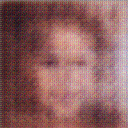
\includegraphics[width=150px]{500_fake_images/samples_5_303.png}%
\caption{A Man Is Taking A Picture Of Himself In The Mirror}%
\end{figure}

%
\end{document}